\documentclass[12pt]{report}
\usepackage{graphicx}
\usepackage[utf8]{inputenc}
\usepackage[spanish]{babel}
\usepackage{setspace}
\usepackage{geometry}
\usepackage{titlesec}
\usepackage{times}
\usepackage{mathptmx} % Use mathptmx instead of times
\usepackage{fancyhdr}



% Configuración de márgenes
\geometry{
    top=2.5cm,
    left=3cm,
    right=3cm,
    bottom=2.5cm
}

% Configuración de interlineado
\onehalfspacing

% Configuración de títulos y subtítulos
\titleformat{\chapter}[display]
  {\normalfont\bfseries\centering}{}{0pt}{\fontsize{14}{16}\selectfont}
\titleformat{\section}
  {\normalfont\bfseries}{\thesection}{1em}{\fontsize{12}{14}\selectfont}
\titleformat{\subsection}
  {\normalfont\bfseries}{\thesubsection}{1em}{\fontsize{12}{14}\selectfont}


% Configuración de pie de página
  \fancyhf{}
\fancyfoot[R]{\thepage}
\pagestyle{fancy}
\fancypagestyle{plain}{
  \fancyhf{}
  \fancyfoot[R]{\thepage}
}

  \begin{document}
  \pagenumbering{roman}
%----- PORTADA ----
\setlength{\hoffset}{27 pt} % 1 (Para centrar más la portada)
\begin{titlepage}
{\centering
{\fontfamily{ptm}\scshape\bfseries\fontsize{29.16}{34.992}\selectfont Universidad de Guadalajara \par}
\vspace{0.5cm}
{\scshape\Large Centro Universitario de los Lagos \par}
\vspace{1cm}
{\scshape\Large División de Estudios de la Biodiversidad e innovación Tecnológica \par}
\vspace{1cm}
{\graphicspath{{imagenes/Portada}} %ruta de las imagenes

\includegraphics[width=0.3\textwidth]{image.png}\par}
\vspace{1cm}
% Título
{\scshape\large\bfseries Resumen Norma IEC 61131\par}
\vspace{1.5cm}
% Materia
{\large \textbf{Materia:} \\Controladores Lógicos Programables\par}
\vfill
% Estudiante
{\large \textbf{Presenta:} \\Oscar Iván Moreno Gutiérrez \#220942754\par}
\vfill
% Profesor
{\large \textbf{Profesor:} \\Dr. Afanador Delgado Samuel Mardoqueo \par}
\vfill
\vfill
% Fecha
\begin{flushright}
  {\normalsize \textbf {Fecha:} \\ \today}
\end{flushright}
\vfill}
{\large  \par}
\end{titlepage}
%----- FIN DE PORTADA ----
\pagenumbering{arabic}

\chapter{Resumen}
Es la base real para estandarizar los lenguajes de programación que se utilizan en la automatización industrial.
El IEC 61131-3 define las especificaciones de la sintaxis y semántica de los lenguajes de PLC, así como su estructura y modelo.
Se generaliza en 2 partes:
\begin{itemize}
  \item Elementos comunes
  \item Lenguajes de programación
\end{itemize}
\begin{figure}[h]
  \centering
  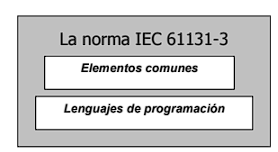
\includegraphics[width=0.5\textwidth]{Imagen_1.png}
  \caption{Partes de IEC 61131-3}
  \label{fig:mi_imagen}
\end{figure}

En los elementos comunes, se definen los tipos de datos. Los tipos de datos previenen errores en una fase inicial.
Los tipos de datos comunes son:
\begin{itemize}
  \item Booleanos
  \item Enteros
  \item Reales
  \item Bytes
  \item Caracteres
  \item Fechas y horas
  \item Cadenas de caracteres
\end{itemize}
También se define si un dato es variable o constante. Si es una variable, esto significa que el valor del dato puede cambiar a través del programa. También se puede especificar si es una variable local o global, lo que significa que su modificación está limitada al ámbito en el que se declara.

Las configuraciones nos permiten controlar problemas específicos, ya que cada configuración es específica para un tipo de sistema de control e incluye las características del hardware.

Dentro de la configuración se definen los recursos, que se entienden como un procesador capaz de ejecutar programas de control escritos en los lenguajes que define la norma.

La norma presenta 3 formas para crear programas de control:
\begin{itemize}
  \item Programas: Conjunto lógico de todos los elementos y construcciones necesarios para el tratamiento de señales requerido para el control de una máquina o proceso mediante un PLC.
  \item Funciones: Las funciones estándar son como ADD, ABS, SQRT, SIN, COS, etc. Las funciones definidas por el usuario se pueden utilizar en cualquier parte del programa una vez implementadas.
  \item Bloques funcionales: Son equivalentes a los circuitos integrados y representan funciones de control especializadas. Estos bloques pueden almacenar información, lo que los diferencia de las funciones. Algunos ejemplos son: biestables, detección de flancos, contadores, temporizadores, etc.
\end{itemize}

Los SFC ayudan a estructurar la organización interna de un programa y a descomponer un problema en partes más pequeñas, manteniendo la estructura completa del programa.
\begin{figure}[h]
  \centering
  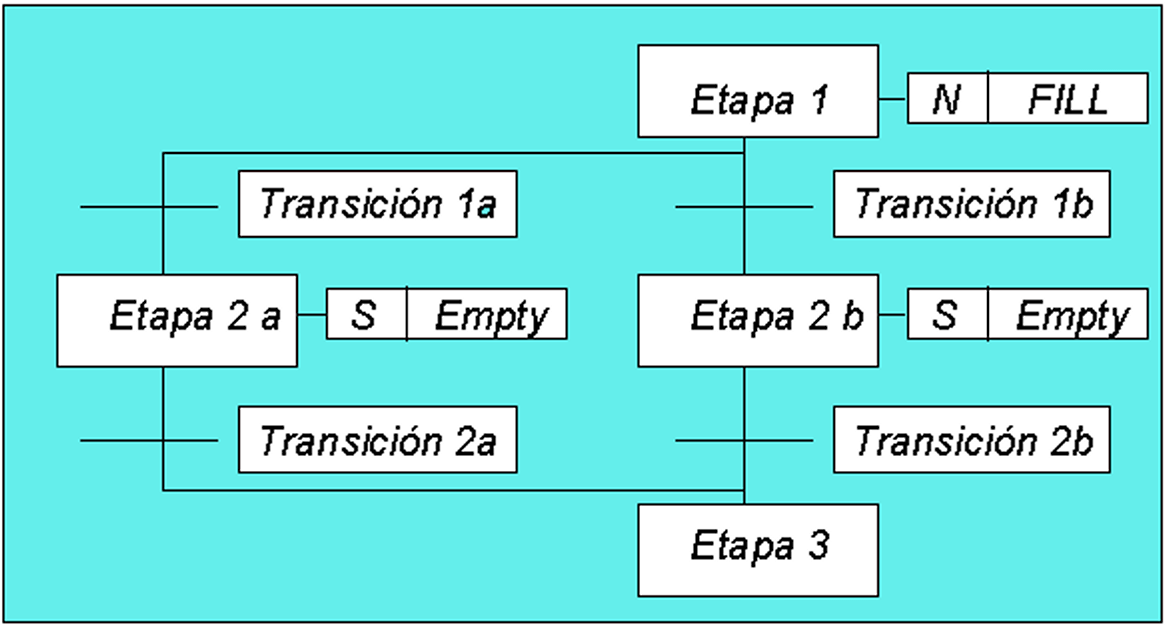
\includegraphics[width=0.5\textwidth]{Imagen_2.png}
  \caption{SFC}
  \label{fig:mi_imagen_2}
\end{figure}

Los lenguajes de programación se dividen en 4, dos de tipo literal y dos de tipo gráfico:
\begin{itemize}
  \item Lenguajes de tipo literal:
  \begin{itemize}
    \item Lenguaje de instrucciones
    \item Lenguaje de texto estructurado
  \end{itemize}
  \item Lenguajes de tipo gráfico:
  \begin{itemize}
    \item Lenguaje de diagrama de bloques
    \item Lenguaje de diagrama de escalera
  \end{itemize}
\end{itemize}
\begin{figure}[h]
  \centering
  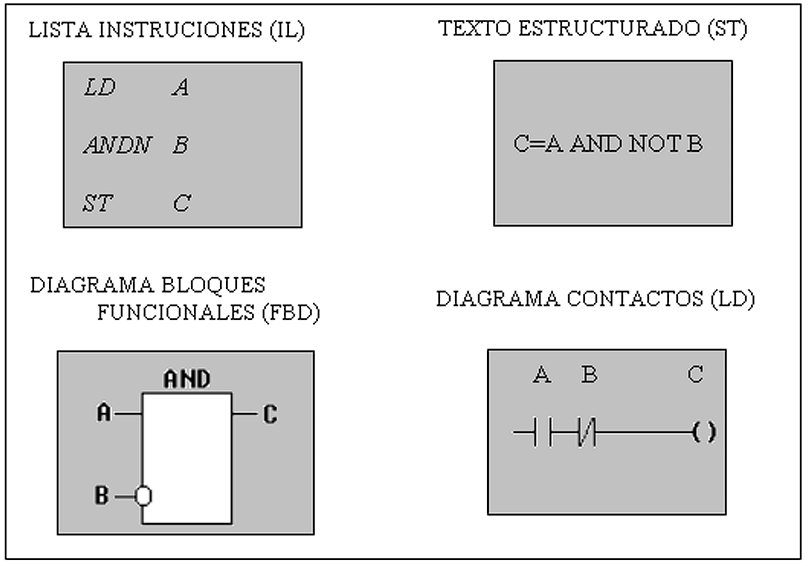
\includegraphics[width=0.5\textwidth]{Imagen_3.png}
  \caption{Lenguajes IEC 61131-3}
  \label{fig:mi_imagen_3}
\end{figure}

Ahora vamos a las formas de desarrollar un programa, hay dos: la primera es Top Down, donde se comienza con los elementos comunes y se avanza hacia el lenguaje. La segunda es Bottom Up, donde se comienza con el lenguaje y se avanza hacia los elementos comunes.
\newpage


%----- PALABRAS CLAVE ----

\chapter*{Palabras Clave}
\begin{itemize}
  \item Controladores Lógicos Programables (PLC): Dispositivos electrónicos utilizados en la automatización industrial para controlar y monitorear procesos.
  \item Lenguajes de programación: Conjunto de lenguajes definidos en la norma IEC 61131-3 que permiten la creación de programas de control en los PLC.
  \item SFC (Sequential Function Chart): Lenguaje gráfico utilizado para estructurar y descomponer programas de control en partes más pequeñas.
  \item Lenguaje de instrucciones: Lenguaje literal utilizado en los programas de control para escribir instrucciones paso a paso.
  \item Lenguaje de texto estructurado: Lenguaje literal estructurado utilizado en los programas de control para escribir instrucciones de forma más legible y organizada.
  \item Lenguaje de diagrama de bloques: Lenguaje gráfico utilizado en los programas de control para representar las funciones y conexiones entre bloques.
  \item Lenguaje de diagrama de escalera: Lenguaje gráfico utilizado en los programas de control para representar las funciones y conexiones mediante contactos y bobinas.
\end{itemize}
\newpage

\end{document}